\section{Descubrimiento de Conocimiento en Base de Datos (KDD)}

El Knowledge Discovery in Databases o KDD, es término ingresado por Usama Fayyad en los años 90’s, el cual, se define como “el proceso no trivial de identificar patrones novedosos, validos, potencialmente útiles y descifrables en el conjunto de datos” [33], siendo uno de los procesos más utilizados a nivel global, dada su generalidad en sus aplicable a distintas áreas, por ejemplo, “marketing finanzas (inversiones específicamente), detección de fraude, manufactura, telecomunicaciones y agentes de internet” [33], donde cada una tiene distinta connotación.

Este proceso consiste en 5 etapas que se describen a continuación [33]:

\begin{itemize}
\item \textbf{Selección}:

\item \textbf{Preprocesamiento}:

\item \textbf{Transformación}:

\item \textbf{Minería de datos}:

\item \textbf{Interpretación y evaluación}:

\end{itemize}

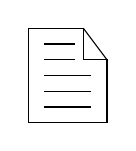
\begin{tikzpicture}
  \draw (0,0) -- (0,1.2) -- (0.7,1.2) -- (0.7,0.8) -- (1,0.8) -- (1,0) -- cycle;
  \draw (0.7,1.2) -- (1,0.8);
  \foreach \y in {0.2,0.4,0.6}{
     \draw (0.2,\y) -- (0.8,\y);
     \draw (0.2,0.8) -- (0.6,0.8);
     \draw (0.2,1) -- (0.6,1);
  }
\end{tikzpicture}

\begin{tikzpicture}[node distance=3cm, auto]

    % Place nodes
    \node[block] (selection) {Seleccion};
    \node[block, right of=selection] (processing) {Procesamiento};
    \node[block, right of=processing] (transformation) {Transformación};
    \node[block, right of=transformation] (data-mining) {Minería de datos};
    \node[block, right of=data-mining] (interpretation) {Interpretación};

\draw[line] (selection) -- (processing)
            (processing) -- (transformation)
            (transformation) -- (data-mining)
            (data-mining) -- (interpretation);

\end{tikzpicture}

\begin{center}
\smartdiagram[descriptive diagram]{
{Set up,The set up operation consist of..},
{Run, {After having set up the program, you must run..}},
{Analyse, You must check what did with analytical tools like..},
{Modify, {After the analysis, you can still modify or add..}},
}
\end{center}
